%===================================================================================
\subsection{CU17 Información del proyecto}
{
\justify
\color{blue}{\textbf{Objetivo}}
}

%------------------------------------------------------------------
\justify
En esta pantalla permite al Lider proyecto podra ver los datos generales del proyecto.
%------------------------------------------------------------------
{
\justify
\color{blue}{\textbf{Diseño}}
}
%-------------------------------------------------------------------------------
\justify
En la figura \ref{fig:IU17} se muestra la pantalla, en donde el Lider de proyecto podrá ver los datos generales del proyecto.

\begin{figure}[htb]
\centering
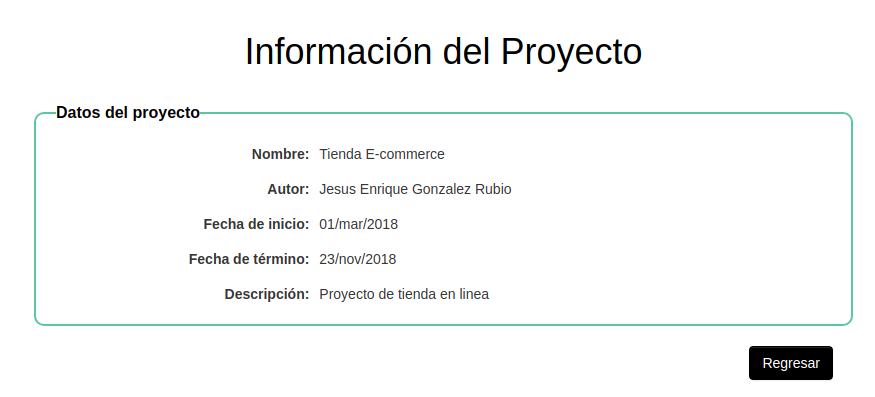
\includegraphics[width=0.8\textwidth]{./images/cu17-informacion-proyecto.png}
\caption{Editar Proyecto.} \label{fig:IU17}
\end{figure}